\documentclass[crop,tikz]{standalone}

\usepackage{tikz}
\usepackage{anyfontsize}
\usetikzlibrary{bending}
\usetikzlibrary{arrows.meta}

\begin{document}

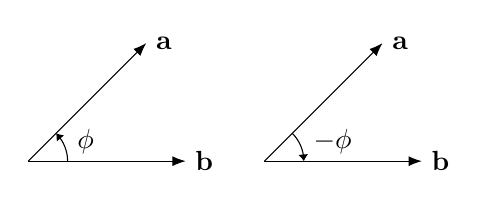
\begin{tikzpicture}
\draw [-Latex] (0,0) -- ++(1.5, 1.5);
\draw [-Latex] (0,0) -- ++(2,0);
\node [right] at (1.5,1.5) {$\bf{a}$};
\node [right] at (2,0) {$\bf{b}$};
\draw [arrows = {-Latex[scale length=0.5]}] ([shift=(0:0.5)]0,0) arc [radius=0.5, start angle=0, end angle= 45];
\node [right] at (0.5, 0.25) {$\phi$};

\draw [-Latex] (3,0) -- ++(1.5, 1.5);
\draw [-Latex] (3,0) -- ++(2, 0);
\node [right] at (4.5,1.5) {$\bf{a}$};
\node [right] at (5, 0) {$\bf{b}$};
\draw [arrows = {-Latex[scale length=0.5]}] ([shift=(45:0.5)]3,0) arc [radius=0.5, start angle=45, end angle= 0];
\node [right] at (3.5, 0.25) {$-\phi$};

\end{tikzpicture}

\end{document}